\subsection{Solución exacta de la ecuación a(e)}
Integrano la ecuación \ref{eq:dade}, encontramos que:
\begin{align*}
    \int_{a_{0}}^{a}\frac{d\bar{a}}{\bar{a}}&=\int_{e_{0}}^{e}\frac{12}{19}\frac{1+(73/24)\bar{e}^2+(37/96)\bar{e}^4}{\bar{e}(1-\bar{e}^2)[1+(121/304)\bar{e}^2]}\,d\bar{e},\\
    \ln \left(\frac{a}{a_{0}}\right)&=\int_{e_{0}}^{e}\frac{12}{19}\frac{1+(73/24)\bar{e}^2+(37/96)\bar{e}^4}{\bar{e}(1-\bar{e}^2)[1+(121/304)\bar{e}^2]}\,d\bar{e}.
\end{align*}
Despejando $a$, obtenemos la expresión
\begin{equation}
    \bar{a}= a_{0}\exp\left[\int_{e_{0}}^{e}\frac{12}{19}\frac{1+(73/24)\bar{e}^2+(37/96)\bar{e}^4}{\bar{e}(1-\bar{e}^2)[1+(121/304)\bar{e}^2]}\,d\bar{e}\right].
    \label{eq:bara}
\end{equation}
Calculando la integral en la expresión anterior con la libreria \textit{sympy} de \textit{python}, se obtiene
\begin{eqnarray*}
        \bar{a}=a_0exp\left[\frac{12}{19}log(e)-\frac{12}{19}log(e_0)-log(e^2-1)+\frac{870}{2299}log\left(e^2+\frac{304}{121}\right)\right.\\
        \left.+log\left(e^2_0-1\right)-\frac{870}{2299}log\left(e^2_0+\frac{304}{121}\right)\right]
\end{eqnarray*}
\begin{equation}
    \bar{a}= \frac{a_0e^{\frac{12}{19}}\left(e^2+\frac{304}{121}\right)^{\frac{870}{2299}}\left(e^2_0-1\right)}{e^{\frac{12}{19}}_0\left(e^2-1\right)\left(e_0^2+\frac{304}{121}\right)^{\frac{870}{2299}}}
\end{equation}
Si definimos a 
\begin{equation}
    g(e):= \frac{e^{\frac{12}{19}}}{1-e^2} \left(1+\frac{121}{304}\right)^{\frac{870}{2299}}
    \label{eq:g(e)}
\end{equation}
entonces, la solución puede escribirse como 
\begin{equation}
    a(e)= a_0\frac{g(e)}{g(e_0)}
    \label{eq:a(e)}
\end{equation}
\subsection{Solución numérica de la función a(e)}
Usando la siguiente adimencionalizació de las variables
\begin{equation*}
    \tilde{a}:= \frac{a}{R_*}, \qquad  \tilde{t}:=\frac{ct}{R_*}.
\end{equation*}
donde
\begin{equation*}
    R_*^3 := \frac{4G^3\mu M^2}{c^6}.
\end{equation*}
Por lo tanto, las ecuaciones \ref{eq:dadt} y \ref{eq:dedt} son:
\begin{align}
    \label{eq:dadt2}
    \frac{d\tilde{a}}{d\tilde{t}} &= -\frac{16}{5}\frac{1}{\tilde{a}^3}\frac{1}{\left(1-e^2\right)^{7/2}}\left(1+\frac{73}{24}e^2+\frac{37}{96}e^4\right) ,\\
    \label{eq:dedt2}
\frac{de}{d\tilde{t}} &= -\frac{76}{15}\frac{1}{\tilde{a}^4}\frac{e}{\left(1-e^2\right)^{5/2}}\left(1+\frac{121}{304}e^2\right) .
\end{align}
Como el sistema de ecuaciones es de primer orden, basta con definir el vector solución $x$ por medio de $x[0]:=\tilde{a}, x[1]=e$. Por lo tanto, 
la ecuación \ref{eq:dadt2} es dada por la función \textcolor{def}{dotx}.
\begin{tcolorbox}[breakable, size=fbox, boxrule=1pt, pad at break*=1mm,colback=cellbackground, colframe=cellborder]
    \prompt{In}{incolor}{*}{\boxspacing}
    \begin{Verbatim}[commandchars=\\\{\}]
    \PY{k}{def} \PY{n+nf}{dotx}\PY{p}{(}\PY{n}{x}\PY{p}{,}\PY{n}{t}\PY{p}{)}\PY{p}{:}
        \PY{n}{a} \PY{o}{=} \PY{n}{x}\PY{p}{[}\PY{l+m+mi}{0}\PY{p}{]}
        \PY{n}{e} \PY{o}{=} \PY{n}{x}\PY{p}{[}\PY{l+m+mi}{1}\PY{p}{]}
        \PY{k}{return} \PY{p}{[}\PY{o}{\PYZhy{}}\PY{p}{(}\PY{l+m+mi}{16}\PY{o}{/}\PY{p}{(}\PY{l+m+mi}{5}\PY{o}{*}\PY{n}{a}\PY{o}{*}\PY{o}{*}\PY{l+m+mi}{3}\PY{p}{)}\PY{p}{)}\PY{o}{*}\PY{p}{(}\PY{l+m+mi}{1}\PY{o}{+}\PY{p}{(}\PY{l+m+mi}{73}\PY{o}{/}\PY{l+m+mi}{24}\PY{p}{)}\PY{o}{*}\PY{n}{e}\PY{o}{*}\PY{o}{*}\PY{l+m+mi}{2}\PY{o}{+}\PY{p}{(}\PY{l+m+mi}{37}\PY{o}{/}\PY{l+m+mi}{96}\PY{p}{)}\PY{o}{*}\PY{n}{e}\PY{o}{*}\PY{o}{*}\PY{l+m+mi}{4}\PY{p}{)}\PY{o}{/}\PY{p}{(}\PY{p}{(}\PY{l+m+mi}{1}\PY{o}{\PYZhy{}}\PY{n}{e}\PY{o}{*}\PY{o}{*}\PY{l+m+mi}{2}\PY{p}{)}\PY{o}{*}\PY{o}{*}\PY{p}{(}\PY{l+m+mi}{7}\PY{o}{/}\PY{l+m+mi}{2}\PY{p}{)}\PY{p}{)}\PY{p}{,}
                \PY{o}{\PYZhy{}}\PY{p}{(}\PY{l+m+mi}{76}\PY{o}{/}\PY{p}{(}\PY{l+m+mi}{15}\PY{o}{*}\PY{n}{a}\PY{o}{*}\PY{o}{*}\PY{l+m+mi}{4}\PY{p}{)}\PY{p}{)}\PY{o}{*}\PY{n}{e}\PY{o}{*}\PY{p}{(}\PY{l+m+mi}{1}\PY{o}{+}\PY{p}{(}\PY{l+m+mi}{121}\PY{o}{/}\PY{l+m+mi}{304}\PY{p}{)}\PY{o}{*}\PY{n}{e}\PY{o}{*}\PY{o}{*}\PY{l+m+mi}{2}\PY{p}{)}\PY{o}{/}\PY{p}{(}\PY{p}{(}\PY{l+m+mi}{1}\PY{o}{\PYZhy{}}\PY{n}{e}\PY{o}{*}\PY{o}{*}\PY{l+m+mi}{2}\PY{p}{)}\PY{o}{*}\PY{o}{*}\PY{p}{(}\PY{l+m+mi}{5}\PY{o}{/}\PY{l+m+mi}{2}\PY{p}{)}\PY{p}{)}\PY{p}{]}
    \end{Verbatim}
    \end{tcolorbox}
    Usando los datos del Pulsar de Hulse y Taulor, de acuerdo a \cite{Weisberg2010}.
    \begin{tcolorbox}[breakable, size=fbox, boxrule=1pt, pad at break*=1mm,colback=cellbackground, colframe=cellborder]
        \prompt{In}{incolor}{*}{\boxspacing}
        \begin{Verbatim}[commandchars=\\\{\}]
        \PY{n}{T0\PYZus{}d} \PY{o}{=} \PY{l+m+mf}{0.322997448911} \PY{c+c1}{\PYZsh{} periodo inicial, en días}
        \PY{n}{e0} \PY{o}{=} \PY{l+m+mf}{0.6171334} \PY{c+c1}{\PYZsh{} excentricidad inicial}
        \PY{n}{M\PYZus{}c} \PY{o}{=} \PY{l+m+mf}{1.3886} \PY{c+c1}{\PYZsh{} masa de la compañera, en masas solares}
        \PY{n}{M\PYZus{}p} \PY{o}{=} \PY{l+m+mf}{1.4398} \PY{c+c1}{\PYZsh{} masa del pulsar, en masas solares}
        \PY{n}{c} \PY{o}{=} \PY{l+m+mi}{299792458} \PY{c+c1}{\PYZsh{} rapidez de la luz, en metros por segundo}
        \PY{n}{MGcm3} \PY{o}{=} \PY{l+m+mf}{4.925490947E\PYZhy{}6} \PY{c+c1}{\PYZsh{} MG/c\PYZca{}3, en segundos}
        \end{Verbatim}
        \end{tcolorbox}
Calculando los parámetros astrofisicos se tiene lo siguiente:
\begin{tcolorbox}[breakable, size=fbox, boxrule=1pt, pad at break*=1mm,colback=cellbackground, colframe=cellborder]
    \prompt{In}{incolor}{*}{\boxspacing}
    \begin{Verbatim}[commandchars=\\\{\}]
    \PY{n}{m\PYZus{}sol} \PY{o}{=} \PY{n}{MGcm3}\PY{o}{*}\PY{n}{c} \PY{c+c1}{\PYZsh{} parametro de masa del Sol m=GM/c\PYZca{}2, en metros}
    \PY{n}{M} \PY{o}{=} \PY{n}{M\PYZus{}c}\PY{o}{+}\PY{n}{M\PYZus{}p} \PY{c+c1}{\PYZsh{} masa total, en masas solares}
    \PY{n}{mu} \PY{o}{=} \PY{p}{(}\PY{n}{M\PYZus{}c}\PY{o}{*}\PY{n}{M\PYZus{}p}\PY{p}{)}\PY{o}{/}\PY{n}{M} \PY{c+c1}{\PYZsh{} masa reducida, en masas solares}
    \PY{n}{R\PYZus{}ast} \PY{o}{=} \PY{n}{m\PYZus{}sol}\PY{o}{*}\PY{p}{(}\PY{l+m+mi}{4}\PY{o}{*}\PY{n}{mu}\PY{o}{*}\PY{n}{M}\PY{o}{*}\PY{o}{*}\PY{l+m+mi}{2}\PY{p}{)}\PY{o}{*}\PY{o}{*}\PY{p}{(}\PY{l+m+mi}{1}\PY{o}{/}\PY{l+m+mi}{3}\PY{p}{)} \PY{c+c1}{\PYZsh{} R\PYZus{}\PYZbs{}ast en metros}
    \PY{n}{T0\PYZus{}s} \PY{o}{=} \PY{n}{T0\PYZus{}d}\PY{o}{*}\PY{l+m+mi}{86400} \PY{c+c1}{\PYZsh{} periodo inicial, en segundos}
    \end{Verbatim}
    \end{tcolorbox}
Definiendo las funciones que relacionan el perioto orbital $T$ (en segundos) con el semieje mayor $a$, y viceversa.
\begin{tcolorbox}[breakable, size=fbox, boxrule=1pt, pad at break*=1mm,colback=cellbackground, colframe=cellborder]
    \prompt{In}{incolor}{*}{\boxspacing}
    \begin{Verbatim}[commandchars=\\\{\}]
    \PY{k}{def} \PY{n+nf}{a}\PY{p}{(}\PY{n}{T\PYZus{}s}\PY{p}{)}\PY{p}{:}
        \PY{k}{return} \PY{p}{(}\PY{n}{m\PYZus{}sol}\PY{o}{*}\PY{n}{M}\PY{o}{*}\PY{p}{(}\PY{n}{c}\PY{o}{*}\PY{n}{T\PYZus{}s}\PY{o}{/}\PY{p}{(}\PY{l+m+mi}{2}\PY{o}{*}\PY{n}{np}\PY{o}{.}\PY{n}{pi}\PY{p}{)}\PY{p}{)}\PY{o}{*}\PY{o}{*}\PY{l+m+mi}{2}\PY{p}{)}\PY{o}{*}\PY{o}{*}\PY{p}{(}\PY{l+m+mi}{1}\PY{o}{/}\PY{l+m+mi}{3}\PY{p}{)}
    
    \PY{k}{def} \PY{n+nf}{T}\PY{p}{(}\PY{n}{a\PYZus{}m}\PY{p}{)}\PY{p}{:}
        \PY{k}{return} \PY{p}{(}\PY{l+m+mi}{2}\PY{o}{*}\PY{n}{np}\PY{o}{.}\PY{n}{pi}\PY{o}{/}\PY{n}{c}\PY{p}{)}\PY{o}{*}\PY{p}{(}\PY{n}{a\PYZus{}m}\PY{o}{*}\PY{o}{*}\PY{l+m+mi}{3}\PY{o}{/}\PY{p}{(}\PY{n}{M}\PY{o}{*}\PY{n}{m\PYZus{}sol}\PY{p}{)}\PY{p}{)}\PY{o}{*}\PY{o}{*}\PY{p}{(}\PY{l+m+mi}{1}\PY{o}{/}\PY{l+m+mi}{2}\PY{p}{)}
        \PY{n}{a0\PYZus{}m} \PY{o}{=} \PY{n}{a}\PY{p}{(}\PY{n}{T0\PYZus{}s}\PY{p}{)} \PY{c+c1}{\PYZsh{} a inicial, en metros}
        \PY{n}{at0} \PY{o}{=} \PY{n}{a0\PYZus{}m}\PY{o}{/}\PY{n}{R\PYZus{}ast} \PY{c+c1}{\PYZsh{} a tilde inicial}
    \end{Verbatim}
    \end{tcolorbox}
Dado que resolveremos el sistema de ecuaciones con distintias condicionesiniciales, definiremos una funcion que nos entrega estas soluciones:
\begin{tcolorbox}[breakable, size=fbox, boxrule=1pt, pad at break*=1mm,colback=cellbackground, colframe=cellborder]
    \prompt{In}{incolor}{*}{\boxspacing}
    \begin{Verbatim}[commandchars=\\\{\}]
    \PY{k}{def} \PY{n+nf}{solucion}\PY{p}{(}\PY{n}{x0}\PY{p}{,}\PY{n}{tt\PYZus{}int}\PY{p}{)}\PY{p}{:}
        \PY{n+nb}{print} \PY{l+s+s1}{\PYZsq{}}\PY{l+s+s1}{Se resuelve con at0 = }\PY{l+s+s1}{\PYZpc{}}\PY{l+s+s1}{2.f y e0 = }\PY{l+s+s1}{\PYZpc{}}\PY{l+s+s1}{2.f}\PY{l+s+s1}{\PYZsq{}}\PY{o}{\PYZpc{}}\PY{p}{(}\PY{n}{x0}\PY{p}{[}\PY{l+m+mi}{0}\PY{p}{]}\PY{p}{,}\PY{n}{x0}\PY{p}{[}\PY{l+m+mi}{1}\PY{p}{]}\PY{p}{)}
        \PY{n}{sol} \PY{o}{=} \PY{n}{odeint}\PY{p}{(}\PY{n}{dotx}\PY{p}{,}\PY{n}{x0}\PY{p}{,}\PY{n}{tt\PYZus{}int}\PY{p}{)}
        \PY{n}{at\PYZus{}todos} \PY{o}{=} \PY{n}{sol}\PY{p}{[}\PY{p}{:}\PY{p}{,}\PY{l+m+mi}{0}\PY{p}{]}
        \PY{c+c1}{\PYZsh{} verifica si at llega a 2. En caso positivo corta el arreglo de soluciones}
        \PY{n}{restriccion} \PY{o}{=} \PY{n}{np}\PY{o}{.}\PY{n}{where}\PY{p}{(}\PY{n}{at\PYZus{}todos}\PY{o}{\PYZlt{}}\PY{l+m+mi}{2}\PY{p}{)}\PY{p}{[}\PY{l+m+mi}{0}\PY{p}{]}
        \PY{k}{if} \PY{n+nb}{len}\PY{p}{(}\PY{n}{restriccion}\PY{p}{)} \PY{o+ow}{is} \PY{o+ow}{not} \PY{l+m+mi}{0}\PY{p}{:}
            \PY{n}{pos\PYZus{}ttmax} \PY{o}{=} \PY{n}{restriccion}\PY{p}{[}\PY{l+m+mi}{0}\PY{p}{]} \PY{c+c1}{\PYZsh{} determina el tiempo en el que at=2}
            \PY{n+nb}{print}\PY{p}{(}\PY{l+s+s1}{\PYZsq{}}\PY{l+s+s1}{Acortando intervalo a tt\PYZus{}max = }\PY{l+s+s1}{\PYZsq{}}\PY{o}{+}\PY{n+nb}{str}\PY{p}{(}\PY{n}{tt\PYZus{}int}\PY{p}{[}\PY{n}{pos\PYZus{}ttmax}\PY{p}{]}\PY{p}{)}\PY{p}{)}
        \PY{k}{else}\PY{p}{:} 
            \PY{n}{pos\PYZus{}ttmax} \PY{o}{=} \PY{n+nb}{len}\PY{p}{(}\PY{n}{tt\PYZus{}int}\PY{p}{)}
        \PY{n}{tt} \PY{o}{=} \PY{n}{tt\PYZus{}int}\PY{p}{[}\PY{p}{:}\PY{n}{pos\PYZus{}ttmax}\PY{p}{]}
        \PY{n}{t\PYZus{}a} \PY{o}{=} \PY{n}{tt}\PY{o}{*}\PY{n}{R\PYZus{}ast}\PY{o}{/}\PY{n}{c}\PY{o}{/}\PY{l+m+mi}{31557600} \PY{c+c1}{\PYZsh{} el tiempo, en años}
        \PY{n}{at} \PY{o}{=} \PY{n}{sol}\PY{p}{[}\PY{p}{:}\PY{n}{pos\PYZus{}ttmax}\PY{p}{,}\PY{l+m+mi}{0}\PY{p}{]}
        \PY{n}{e} \PY{o}{=} \PY{n}{sol}\PY{p}{[}\PY{p}{:}\PY{n}{pos\PYZus{}ttmax}\PY{p}{,}\PY{l+m+mi}{1}\PY{p}{]}
        \PY{n}{a\PYZus{}m} \PY{o}{=} \PY{n}{at}\PY{o}{*}\PY{n}{R\PYZus{}ast} \PY{c+c1}{\PYZsh{} solución de a, en metros}
        \PY{n}{T\PYZus{}s} \PY{o}{=} \PY{n}{T}\PY{p}{(}\PY{n}{a\PYZus{}m}\PY{p}{)} \PY{c+c1}{\PYZsh{} solución de T, en segundos}
        \PY{k}{return} \PY{n}{tt}\PY{p}{,}\PY{n}{t\PYZus{}a}\PY{p}{,}\PY{n}{at}\PY{p}{,}\PY{n}{e}\PY{p}{,}\PY{n}{a\PYZus{}m}\PY{p}{,}\PY{n}{T\PYZus{}s}
    \end{Verbatim}
    \end{tcolorbox}
Al realizar tener la solución de a ecuación adimensionada, los valores son del orden de 10\textsuperscript{21} para que el sistema 
colapse, se transformo para que cada solución tenga dimensiones, por lo que al graficar el semieje mayor a y la excentricidad con respecto el tiempo obtememos la figura
\ref{fig:semieje,excentricidad}.
\begin{figure}[H]
    \centering
    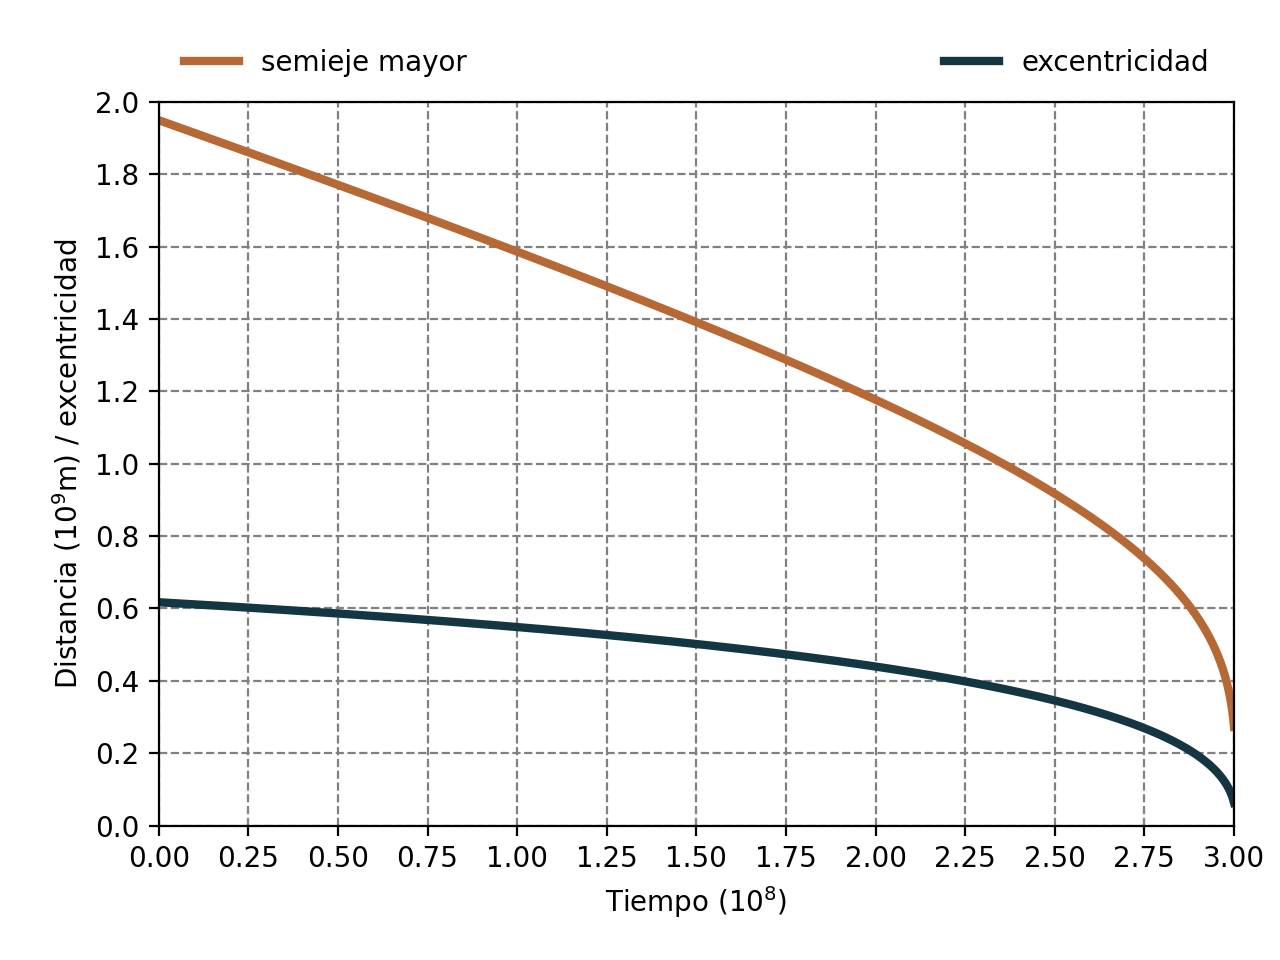
\includegraphics[scale=0.75]{images/a_adim.png}
    \caption{Semieje mayor y la excentricidad de la dinámica del pulsar binario a lo largo del tiempo.}
    \label{fig:semieje,excentricidad}
\end{figure}
Obteniendo el periodo orbital en horas del sistema obtenemos la figura \ref{fig:periodo}.
\begin{figure}[H]
    \centering
    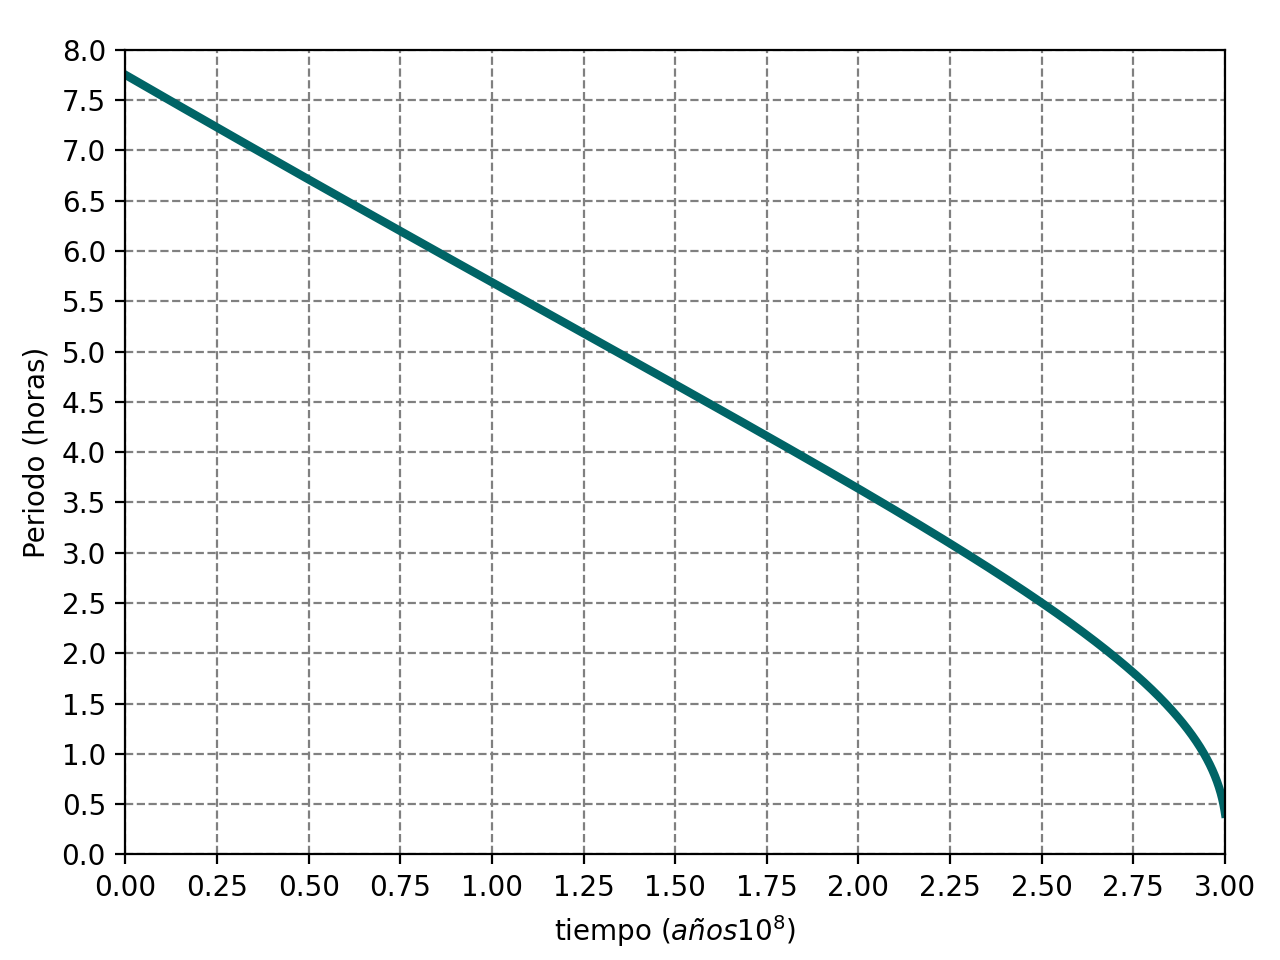
\includegraphics[scale=0.75]{images/periodo.png}
    \caption{Periodo orbital en horas del sistema binario con respecto el tiempo en años.}
    \label{fig:periodo}
\end{figure}
Al tener los valores que contiene la excentricidad de la órbita del sistema, entonces podemos visualizar la forma de la funcion \ref{eq:g(e)}, esta 
función propuesta es la que se visualiza en la figura \ref{fig:gvse}.
\begin{figure}[H]
    \centering
    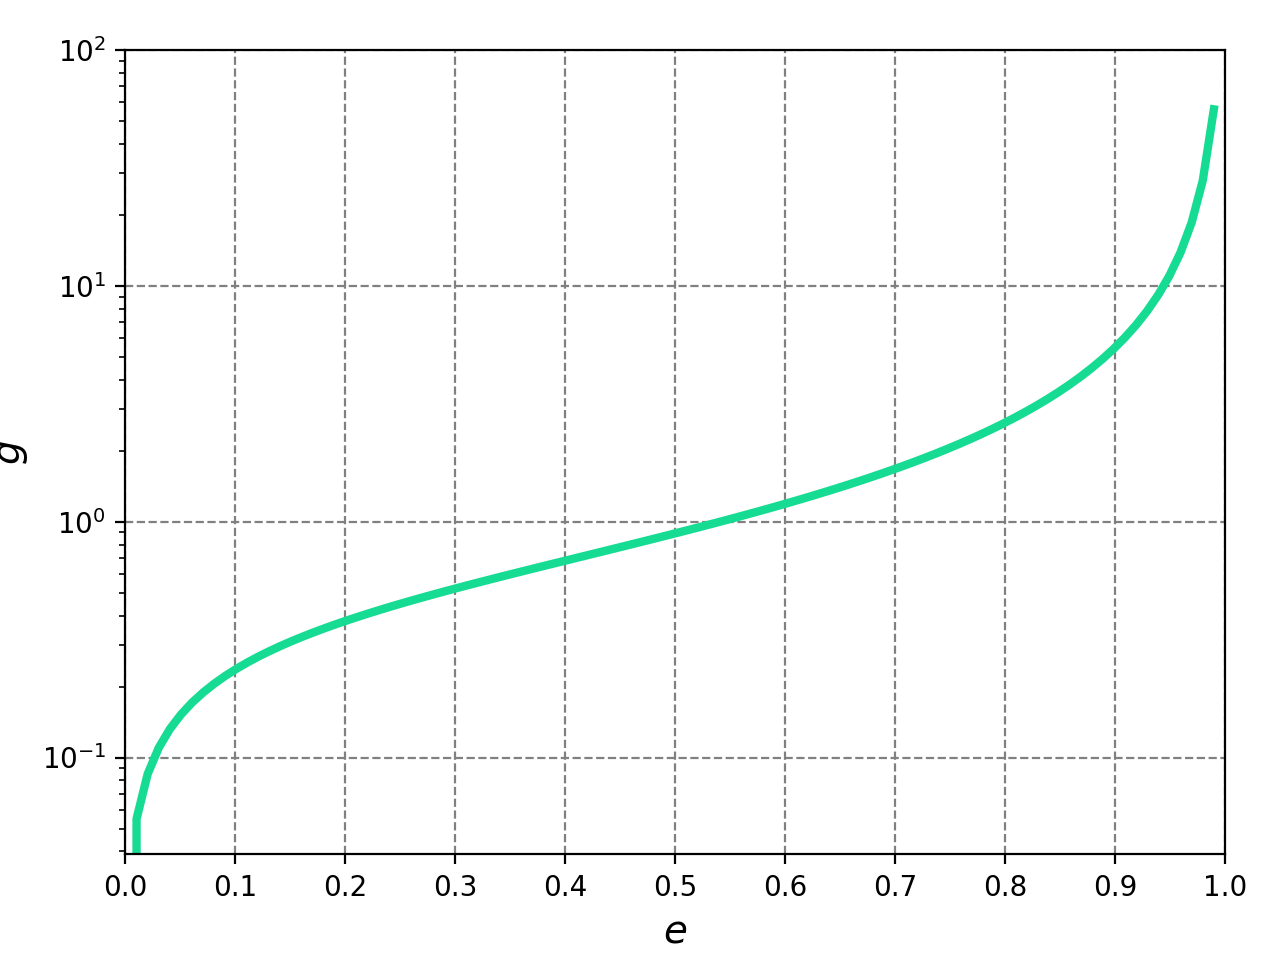
\includegraphics[scale=0.75]{images/gvse.png}
    \caption{Función g(e) con respecto los valores de la excentricidad calculados.}
    \label{fig:gvse}
\end{figure}
Ahora graficando los valores del semieje mayor $a$ con respecto a los valores de la excentricidad $e$, tanto para la solución análitica y númerica se obtiene la figura
\ref{fig:ananum}
\begin{figure}[H]
    \centering
    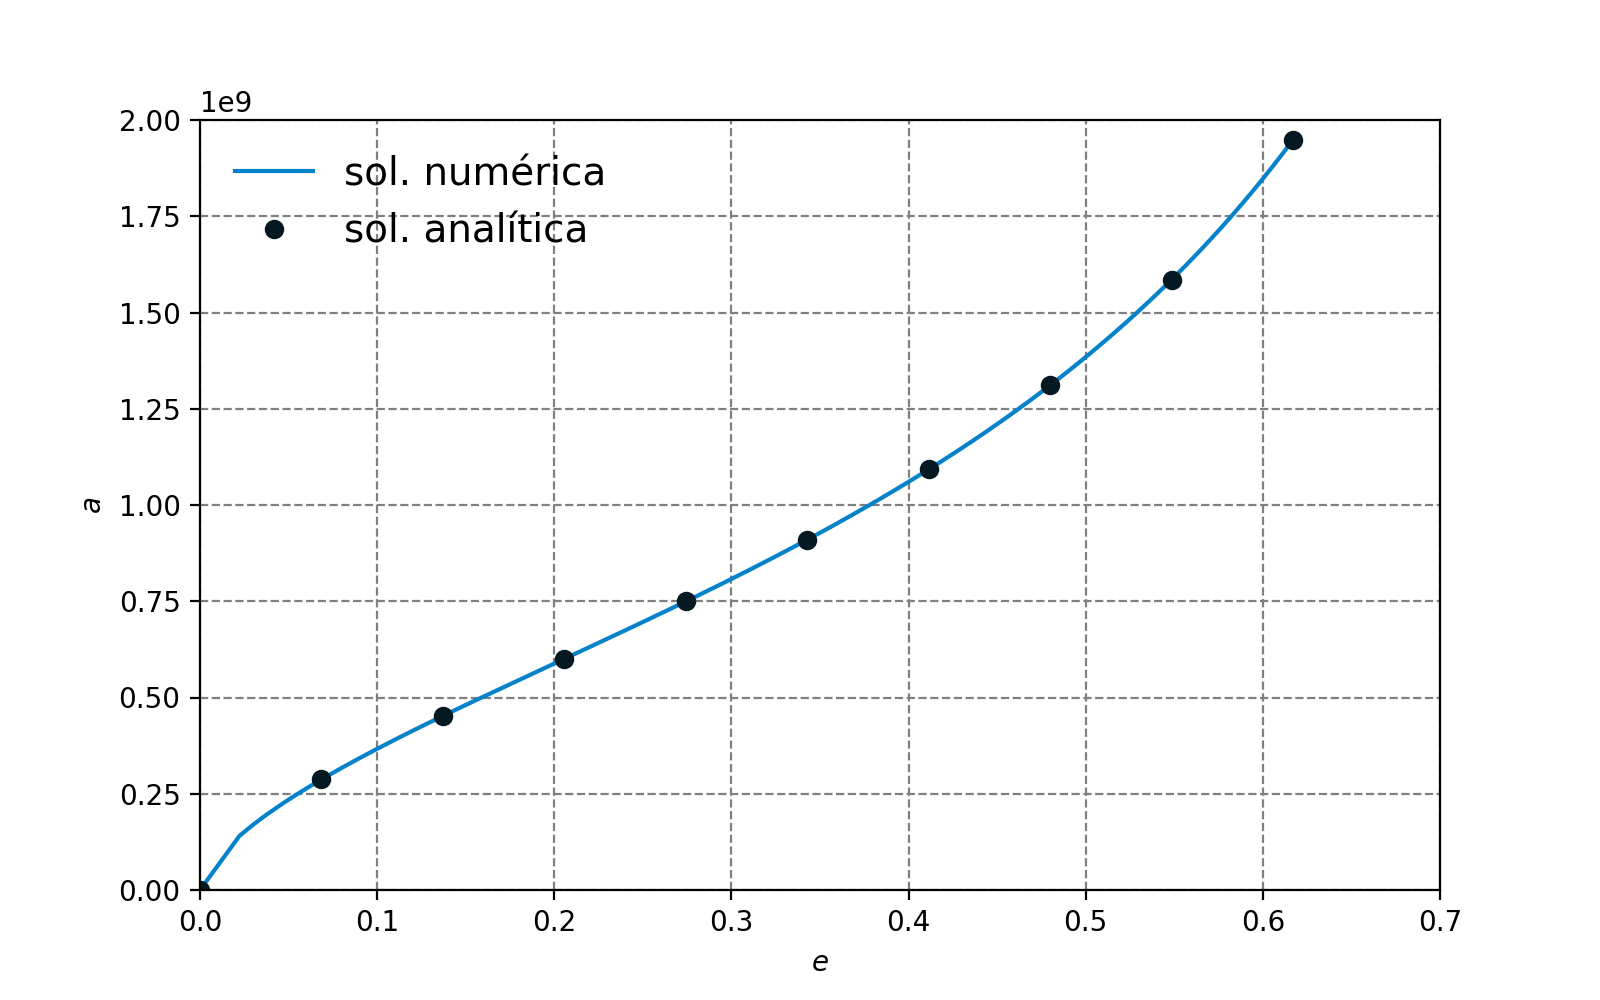
\includegraphics[scale=0.75]{images/solana_solnum.png}
    \caption{Valores del semieje mayor $a$ con respecto a los valores de excentricidad $e$ para la solución análitica u numérica.}
    \label{fig:ananum}
\end{figure}
Este comportamiento implica que en este intervalo de tiempo de aproximadamente 30 años los valores de $\dot{T}$, $\dot{a}$ y $\dot{e}$ pueden considerarse constantes. Con el valor de $\dot{T}$ podemos modelar el retardo acumulado en el movimiento orbital del sistema. Si $\dot{T}=$ cte. entonces el tiempo transcurrido hasta completar la $n$-ésima revolución es determinado por las relaciones
\begin{align*}
T(t)&\approx T_0 + \dot{T}(t-t_0),\\
t_{n+1}& \approx t_n + T(t_n).
\end{align*}
que al ser iteradas implican que
\begin{equation*}
t_n \approx t_0+nT_0+\dot{T}T_0\frac{n(n-1)}{2}+O(\dot{T}{}^2).
\end{equation*}
Por lo tanto, el retardo respecto al valor newtoniano ($t_n^{\rm Newton}=t_0+nT_0$), luego de $n$ revoluciones es dado por
\begin{equation*}
(\Delta t)_n \approx \dot{T}T_0\frac{n(n-1)}{2}+O(\dot{T}{}^2).
\end{equation*}

El valor de $\dot{T}$ puede ser evaluado usando la función dotx que definimos previamente, y con la relación
\begin{equation*}
\dot{T}=\frac{3}{2}\frac{c}{R_\ast}\frac{T}{\tilde{a}}\frac{d\tilde{a}}{d\tilde{t}}
\end{equation*}
Obteniendo un valor de 
\begin{equation*}
    \frac{dT}{dt}=-2.402560x10^{-12}
\end{equation*}
Este valor concuerda con el reportado en \cite{Weisberg2010}. Por lo que comparando los datos observacionales con los teóricos obtenemos la figura \ref{fig:exp}
\begin{figure}[H]
    \centering
    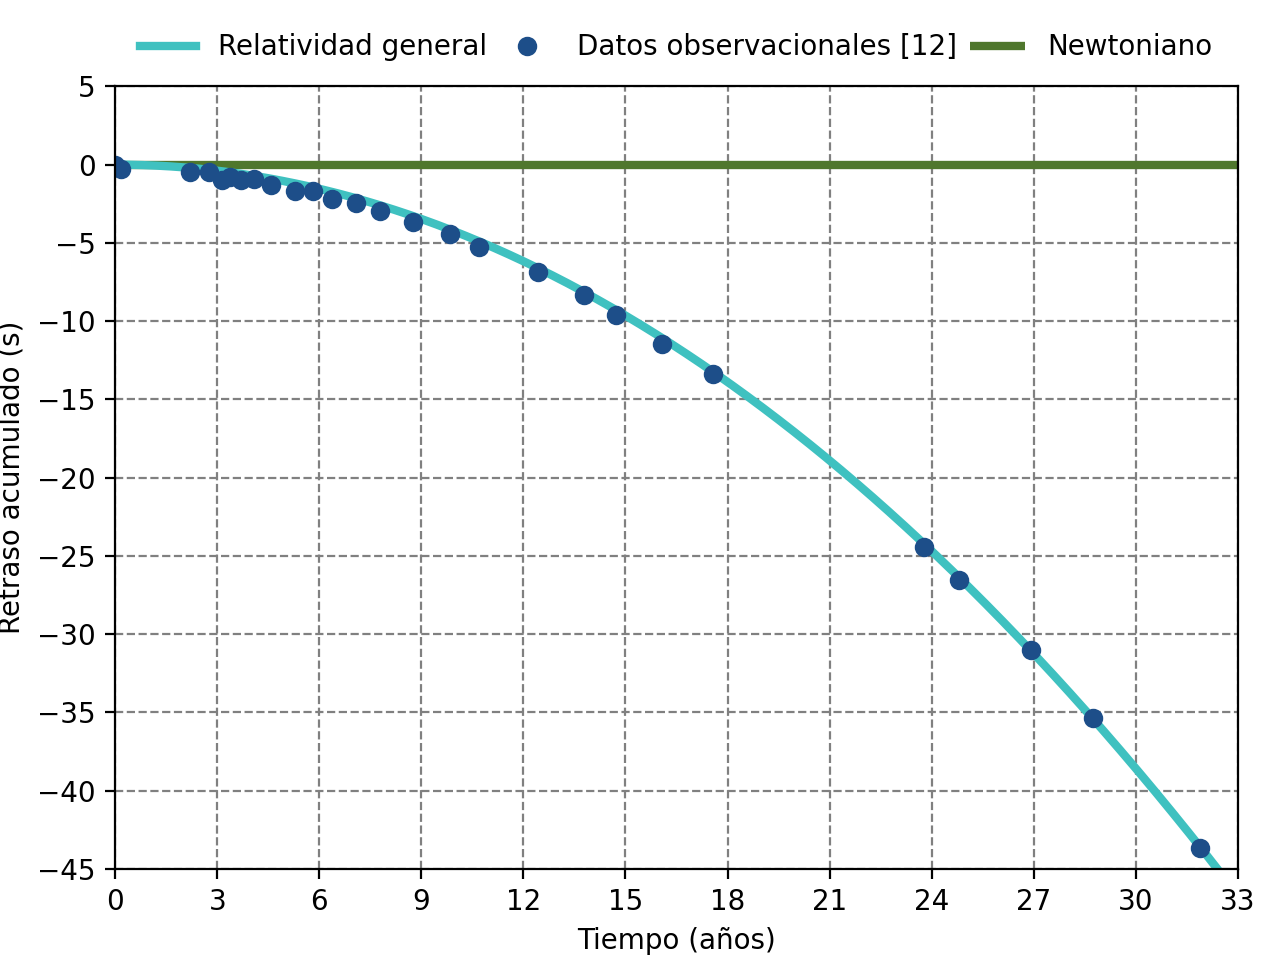
\includegraphics[scale=0.75]{images/exp.png}
    \caption{Datos observacionales reportados en \cite{Weisberg2010} comparados con la solución teórica aportada por la relatividad general y la teoría newtoniana.}
    \label{fig:exp}
\end{figure}